\documentclass[14pt]{extbook}
\usepackage{multicol, enumerate, enumitem, hyperref, color, soul, setspace, parskip, fancyhdr} %General Packages
\usepackage{amssymb, amsthm, amsmath, bbm, latexsym, units, mathtools} %Math Packages
\everymath{\displaystyle} %All math in Display Style
% Packages with additional options
\usepackage[headsep=0.5cm,headheight=12pt, left=1 in,right= 1 in,top= 1 in,bottom= 1 in]{geometry}
\usepackage[usenames,dvipsnames]{xcolor}
\usepackage{dashrule}  % Package to use the command below to create lines between items
\newcommand{\litem}[1]{\item#1\hspace*{-1cm}\rule{\textwidth}{0.4pt}}
\pagestyle{fancy}
\lhead{Makeup Progress Quiz 3}
\chead{}
\rhead{Version C}
\lfoot{4315-3397}
\cfoot{}
\rfoot{Fall 2020}
\begin{document}

\begin{enumerate}
\litem{
Choose the equation of the function graphed below.
\begin{center}
    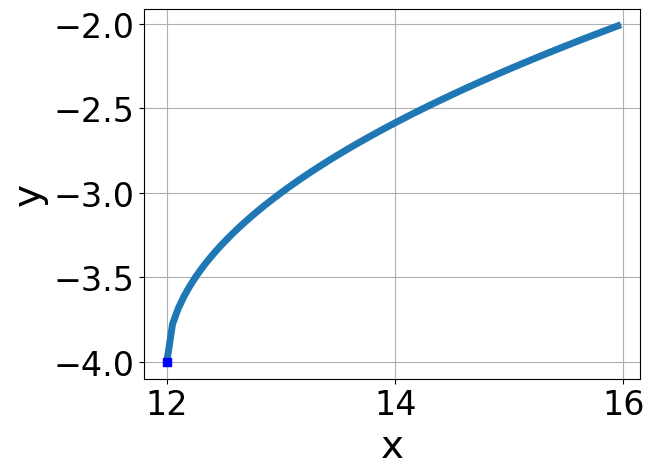
\includegraphics[width=0.5\textwidth]{../Figures/radicalGraphToEquationCopyC.png}
\end{center}
\begin{enumerate}[label=\Alph*.]
\item \( f(x) = \sqrt{x + 12} - 4 \)
\item \( f(x) = - \sqrt{x + 12} - 4 \)
\item \( f(x) = \sqrt{x - 12} - 4 \)
\item \( f(x) = - \sqrt{x - 12} - 4 \)
\item \( \text{None of the above} \)

\end{enumerate} }
\litem{
What is the domain of the function below?\[ f(x) = \sqrt[4]{5 x - 7} \]\begin{enumerate}[label=\Alph*.]
\item \( (-\infty, \infty) \)
\item \( (-\infty, a], \text{where } a \in [1.16, 1.84] \)
\item \( [a, \infty), \text{ where } a \in [1.27, 1.56] \)
\item \( (-\infty, a], \text{where } a \in [-0.5, 0.82] \)
\item \( [a, \infty), \text{where } a \in [-0.14, 1.01] \)

\end{enumerate} }
\litem{
Solve the radical equation below. Then, choose the interval(s) that the solution(s) belongs to.\[ \sqrt{8 x - 2} - \sqrt{3 x - 3} = 0 \]\begin{enumerate}[label=\Alph*.]
\item \( x_1 \in [-0.4, 0.02] \text{ and } x_2 \in [-1.12,0.42] \)
\item \( x \in [0.76,1.43] \)
\item \( x \in [-0.4,0.02] \)
\item \( x_1 \in [0.24, 0.59] \text{ and } x_2 \in [0.9,1.31] \)
\item \( \text{All solutions lead to invalid or complex values in the equation.} \)

\end{enumerate} }
\litem{
Choose the graph of the equation below.\[ f(x) = \sqrt[3]{x + 6} + 3 \]\begin{enumerate}[label=\Alph*.]
\begin{multicols}{2}\item 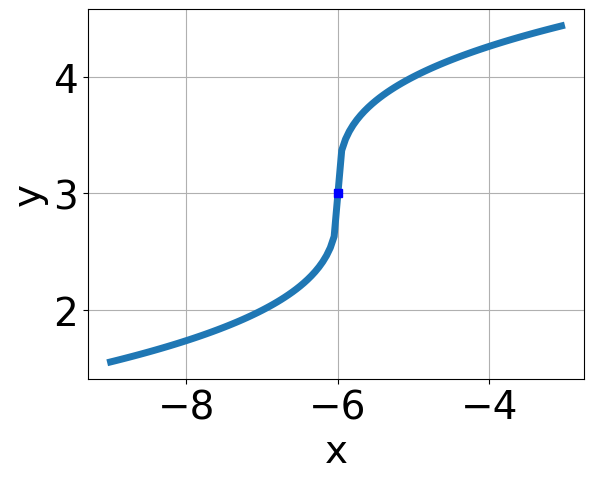
\includegraphics[width = 0.3\textwidth]{../Figures/radicalEquationToGraphAC.png}\item 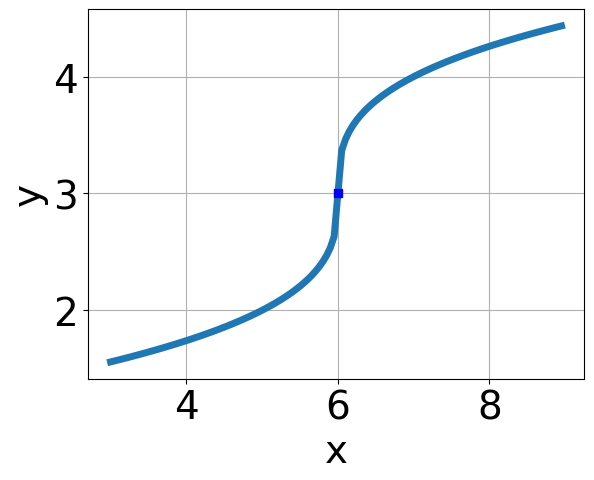
\includegraphics[width = 0.3\textwidth]{../Figures/radicalEquationToGraphBC.png}\item 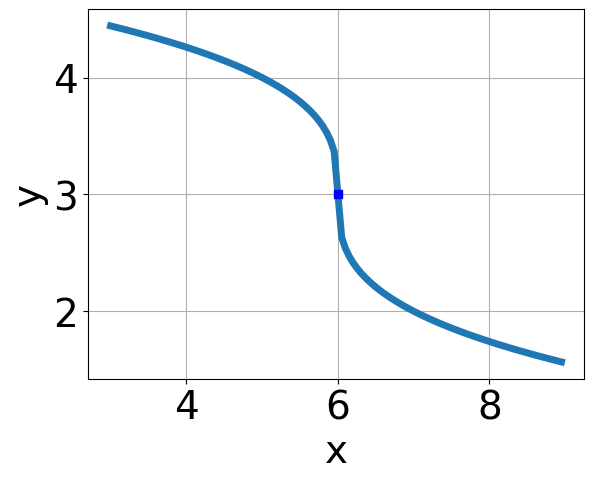
\includegraphics[width = 0.3\textwidth]{../Figures/radicalEquationToGraphCC.png}\item 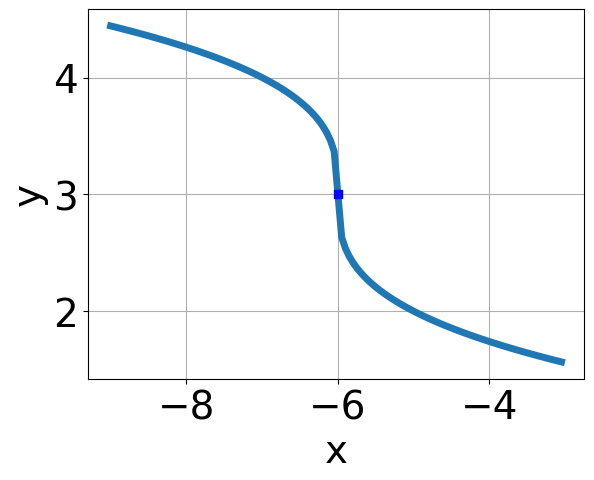
\includegraphics[width = 0.3\textwidth]{../Figures/radicalEquationToGraphDC.png}\end{multicols}\item None of the above.
\end{enumerate} }
\litem{
What is the domain of the function below?\[ f(x) = \sqrt[4]{4 x - 6} \]\begin{enumerate}[label=\Alph*.]
\item \( [a, \infty), \text{where } a \in [0.19, 1.17] \)
\item \( (-\infty, \infty) \)
\item \( [a, \infty), \text{ where } a \in [1.26, 2.09] \)
\item \( (-\infty, a], \text{where } a \in [-0.9, 1.18] \)
\item \( (-\infty, a], \text{where } a \in [1.38, 2.32] \)

\end{enumerate} }
\litem{
Choose the graph of the equation below.\[ f(x) = \sqrt[3]{x + 6} - 7 \]\begin{enumerate}[label=\Alph*.]
\begin{multicols}{2}\item 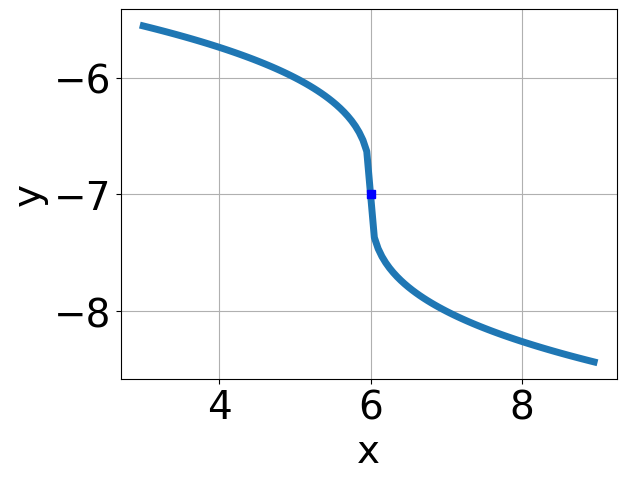
\includegraphics[width = 0.3\textwidth]{../Figures/radicalEquationToGraphCopyAC.png}\item 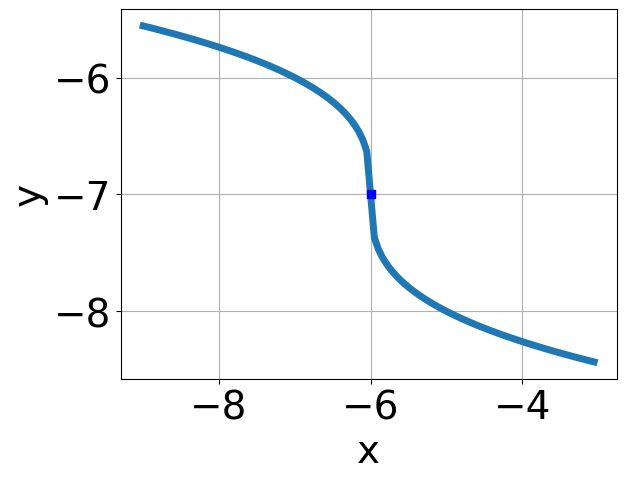
\includegraphics[width = 0.3\textwidth]{../Figures/radicalEquationToGraphCopyBC.png}\item 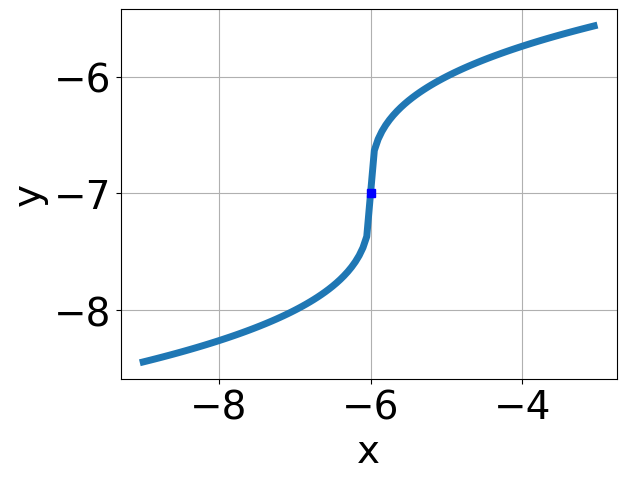
\includegraphics[width = 0.3\textwidth]{../Figures/radicalEquationToGraphCopyCC.png}\item 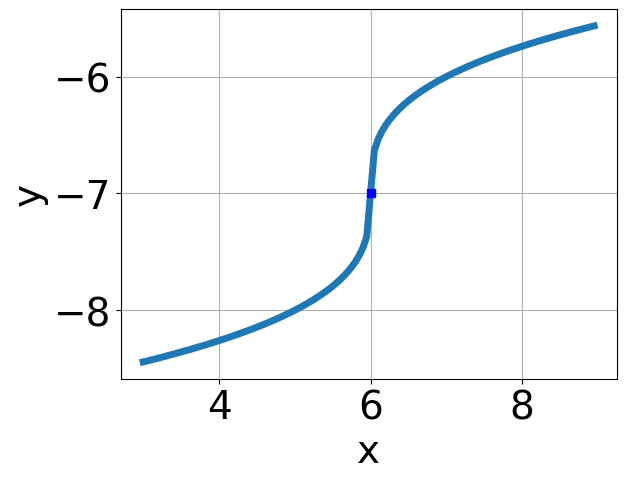
\includegraphics[width = 0.3\textwidth]{../Figures/radicalEquationToGraphCopyDC.png}\end{multicols}\item None of the above.
\end{enumerate} }
\litem{
Solve the radical equation below. Then, choose the interval(s) that the solution(s) belongs to.\[ \sqrt{15 x^2 - 8} - \sqrt{2 x} = 0 \]\begin{enumerate}[label=\Alph*.]
\item \( x_1 \in [-1.08, -0.65] \text{ and } x_2 \in [-0.2,2.8] \)
\item \( \text{All solutions lead to invalid or complex values in the equation.} \)
\item \( x \in [-1.08,-0.65] \)
\item \( x_1 \in [0.3, 0.69] \text{ and } x_2 \in [-0.2,2.8] \)
\item \( x \in [0.67,1.17] \)

\end{enumerate} }
\litem{
Solve the radical equation below. Then, choose the interval(s) that the solution(s) belongs to.\[ \sqrt{-30 x^2 + 16} - \sqrt{4 x} = 0 \]\begin{enumerate}[label=\Alph*.]
\item \( x_1 \in [-1.1, 0.5] \text{ and } x_2 \in [0.11,0.74] \)
\item \( \text{All solutions lead to invalid or complex values in the equation.} \)
\item \( x \in [-0.2,3.2] \)
\item \( x \in [-1.1,0.5] \)
\item \( x_1 \in [-0.2, 3.2] \text{ and } x_2 \in [0.76,1.16] \)

\end{enumerate} }
\litem{
Solve the radical equation below. Then, choose the interval(s) that the solution(s) belongs to.\[ \sqrt{-4 x - 8} - \sqrt{-5 x + 4} = 0 \]\begin{enumerate}[label=\Alph*.]
\item \( x \in [12,15] \)
\item \( x \in [1,11] \)
\item \( x_1 \in [-2, 3] \text{ and } x_2 \in [0.8,3.8] \)
\item \( \text{All solutions lead to invalid or complex values in the equation.} \)
\item \( x_1 \in [-2, 3] \text{ and } x_2 \in [10,14] \)

\end{enumerate} }
\litem{
Choose the equation of the function graphed below.
\begin{center}
    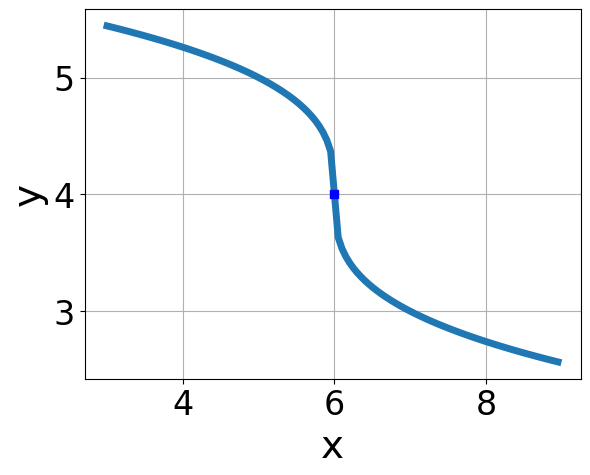
\includegraphics[width=0.5\textwidth]{../Figures/radicalGraphToEquationC.png}
\end{center}
\begin{enumerate}[label=\Alph*.]
\item \( f(x) = \sqrt[3]{x - 6} + 4 \)
\item \( f(x) = \sqrt[3]{x + 6} + 4 \)
\item \( f(x) = - \sqrt[3]{x - 6} + 4 \)
\item \( f(x) = - \sqrt[3]{x + 6} + 4 \)
\item \( \text{None of the above} \)

\end{enumerate} }
\end{enumerate}

\end{document}